\subsubsection{Android}

Le développement d'une application Android s'effectue généralement en utilisant le Java ainsi qu'Android Studio \cite{androidstudio}, permettant d'inclure les bibliothèques Android. Ici, nous avons donc utilisé ces technologies pour permettre une intégration parfaite sur les systèmes Android.

Android est un système d’exploitation à destination des plateformes mobiles supporté par Google et basé sur un noyau Linux. Il équipe aujourd’hui plus de 80\% des terminaux mobiles mais s’adapte aussi sur une large gamme de produits : smartphones, tablettes, montres, téléviseurs, etc. Les systèmes Android sont capables d’exécuter des programmes dérivés du Java grâce à leur environnement d’exécution : une machine virtuelle Dalvik ou l’Android Runtime selon la version. Il est donc possible de produire des exécutables de type apk à base de Java en s’appuyant sur le SDK Android, à la rédaction de ce rapport l’API la plus récente est la 25.

La programmation Android est donc très proche du développement d’applications Java modernes mais comporte tout de même des concepts spécifiques apportées par le SDK. On peut citer par exemple le concept d’activité qui représente une vue dans une application ou encore un intent qui est une demande de service qu’une application peut envoyer au système. L’API propose aussi une pléthore de fonctionnalités utilisant les composants du terminal mobile : gps, accéléromètre, appels réseaux, contacts, sms, etc.

En plus du SDK Android, notre projet nécessite l’utilisation de trois autres bibliothèques : les Google Services, Volley et OpenGL ES. 

Le premier, les Google Services, est un ensemble de fonctionnalités avancées fournies par Google. Les Google Services permettent à tous ceux utilisant un terminal Android d’accéder aux dernières fonctionnalités sans pour autant avoir la dernière version de l’OS. La subtilité derrière ces services est qu’officiellement, Android est censé être un système open source, toutefois pour garder la maitrise du produit Google a décidé de freiner sa participation au cœur d’Android et propose ses meilleurs services et évolutions au travers des Google Services ce qui leur permet de rendre Android presque totalement dépendant de Google. Le géant américain participe donc de façon fermée à un projet open source en empêchant toute concurrence. Dans le cadre de ce projet c’est le système de géolocalisation amélioré qui nous intéresse dans ces services. En effet, la version Android fourni juste la position donnée par le capteur alors que les Google Services prennent en compte plusieurs paramètres comme l’historique de position, les mouvements, les déplacements, etc.

La bibliothèque Volley permet d’effectuer des requêtes réseaux avec une plus grande facilité. Comme on peut le voir sur la figure \ref{volley}, Volley est capable d’exécuter des appels asynchrones et de cacher les réponses. Les gains en performances et en expérience utilisateur sont donc tout à fait de la partie.

\begin{figure}[H]
    \centering
    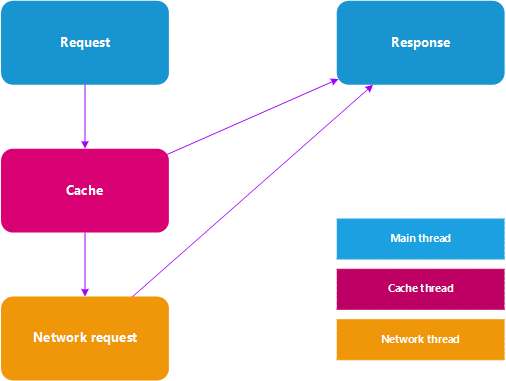
\includegraphics[height=8cm]{./img/volley.png}
    \caption{Fonctionnement d’un requête Volley}
    \label{volley}
\end{figure}

Cette bibliothèque apporte donc des fonctionnalités d’un peu plus haut niveau que le basic HttpUrlConnection de java.net si l’on considère les appels implicites à d’autres threads et des performances améliorées grâce au caching (pour le chargement d’images par exemple).

Enfin le dernier framework utilisé est OpenGL ES ou Embedded System. Ce n’est autre que la version portable du célèbre framework graphique qui a été conçu spécialement pour la programmation embarquée. Comme son ainée, cette version dispose d’une API de bas niveau mais permet au moins de réaliser énormément de choses. En effet il aurait été possible d’utiliser le framework Unity (haut niveau) comme beaucoup d’applications 3D le font, mais cela implique d’utilise des ressources propriétaires payantes alors que les vues 3D à développer dans notre cas ne sont pas très évoluées.

La dernière technologie à présenter en lien direct avec Android est bien sûr l’IDE utilisé. Nous avons opté pour Android Studio, visible sur la figure \ref{androidstudio}, qui est l’environnement de développement officiel d’Android. Android Studio s’inspire grandement des autres outils de la société JetBrains en intégrant beaucoup d’utilitaires spécifiques au développement Android. Il existe d’autres solution comme des versions ou même des plugins Eclipse mais depuis l’arrivée en 2014 d’Android Studio, il n’est vraiment pas recommandé d’utiliser encore Eclipse. Un autre, Processing permet d’effectuer du développement Android mais on est quand même loin de l’outil de JetBrains au niveau des fonctionnalités.

\begin{figure}[H]
    \centering
    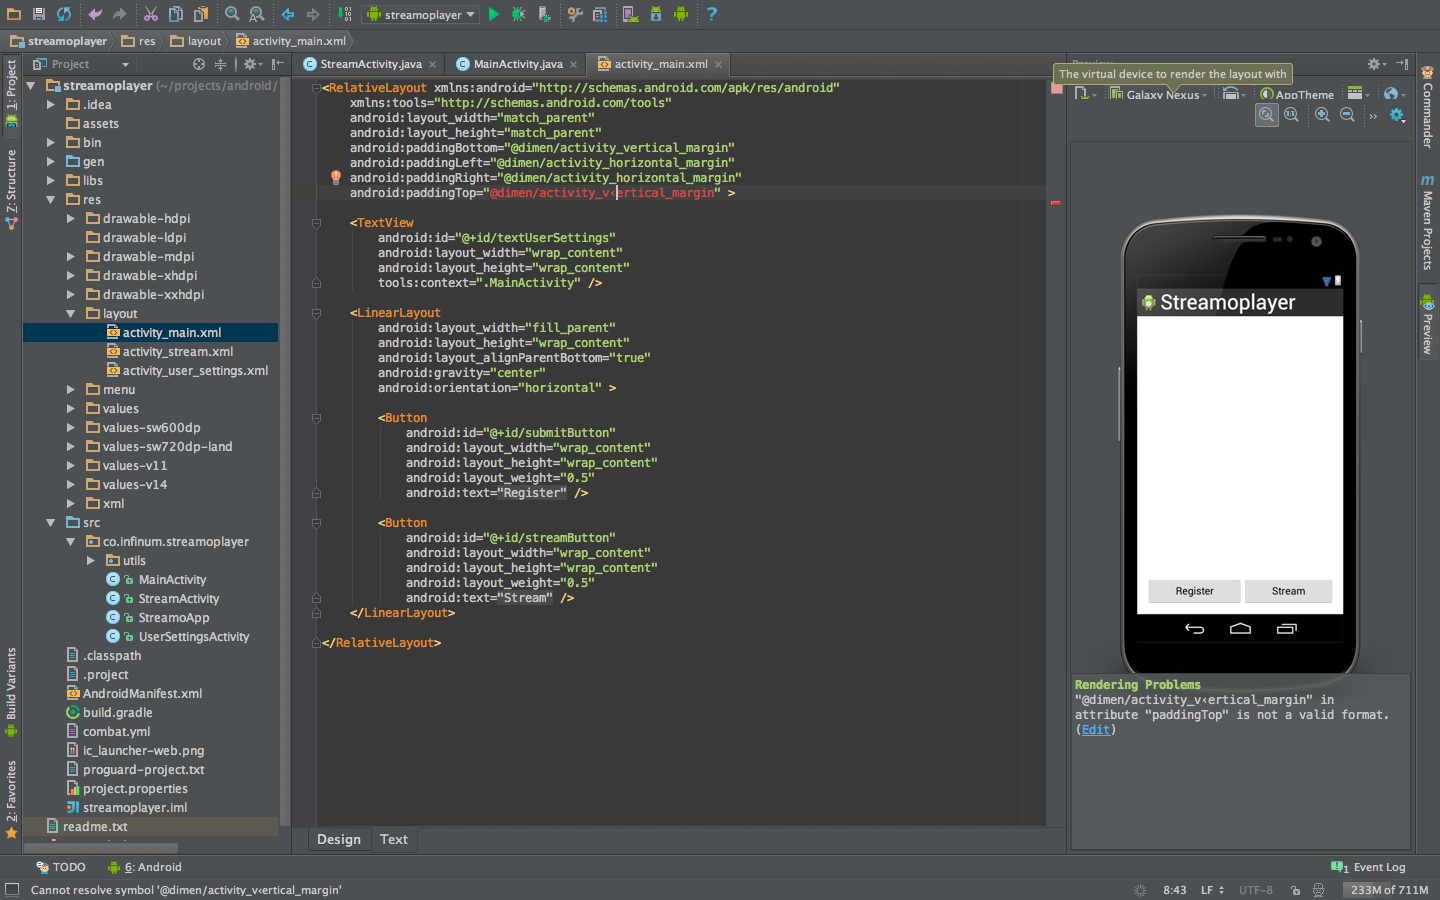
\includegraphics[width=\textwidth]{./img/android-studio.png}
    \caption{Environnement de développement intégré officiel d’Android}
    \label{androidstudio}
\end{figure}

Nous n’allons pas passer en revue ici toutes les fonctionnalités d’Android Studio qui comporte bien sûr toutes les fonctionnalités que l’on peut attendre d’un environnement professionnel mais il faut remarquer qu’il dispose d’outils remarquables.

Le premier est son gestionnaire de SDK : celui-ci permet de maintenir à jour et de manipuler toutes les versions de SDK disponibles. C’est plutôt utile pour un développement où chaque client est différent même si cela reste de l’Android.

Le second est la mise à disposition d’émulateurs Android. Il permet de simuler des terminaux Android de toutes sortes sans besoin de disposer du matériel en réalité. De plus le moniteur intégré permet de suivre en détail l’activité du simili-système ce qui est un plus lors de l’analyse d’exécution d’une application.

Enfin, Android Studio permet de développer les interfaces graphiques soit en mode texte soit en mode WYSIWYG ce qui peut avoir l’avantage d’avoir une prévisualisation d’une vue sans avoir à exécuter toute l’application.

Nous allons maintenant aborder les technologies tierces utilisées au cours de ce projet.